\chapter{Dynamic OpenCL}

\section{Distribution Approach}
\label{distribution}
As portrayed in section \ref{distribution_basics} and \ref{related} many viable options exist to distribute tasks among devices within a single machine as well as across a cluster. This section will explain the reasons for selecting the fitting approaches based on the goals declared in section \ref{goals}.

At first it is important to evaluate the options for running tasks on multiple devices within a single machine. While low level solutions like OpenMP or OpenACC are matured, they add considerable overhead to programming efforts. All communication and synchronization across multiple cores and devices has to be handled by the programmer, which adds introduces a layer of complexity through the utilization of directives. Thus, programmers have to be knowledgable and experiences in utilizing these directives for an efficient execution.

Instead OpenCL will be selected for the distribution of tasks within a single machine. While CUDA offers similar capabilities as OpenCL, it only supports NVIDIA GPUs and completely lacks CPU support. This contradicts with the proposed goal of a heterogenous environment in which devices of different types and vendors cooperate. OpenCL introduces a standardized form in which algorithms have to be designed following the defined memory model and work-item approach. Even though many synchronization and communication calls like data transfers are abstracted away from the programmer, significant low level knowledge is required for building algorithms in the framework. In order to create a more simplified approach, difficult issues for programmers should also be abstracted behind a meaningful API. The necessary steps for that are covered in section \ref{abstraction}.

Even though many solutions for distributing computational workloads among machines in a cluster, most require significant cluster management or programming efforts. Because OpenCL is selected as the underlying computational framework on the machines, the cluster distribution technology has to fit its capabilities.

Similar to OpenMP, MPI has matured over decades as a standard solution for low level communications between multiple machines. As such it has also been used frequently in conjunction with OpenCL and inspired frameworks to build upon this combination. Still, MPI remains a significant contributor to program complexity.

On the opposite MapReduce based frameworks like Hadoop MapReduce offer a strict programming model with a fixed API to follow for each implemented algorithm. As such it has also been used to run OpenCL on top of it within Map phases. In addition some solutions were created by researchers utilizing both technologies in conjunction. As Hadoop MapReduce requires HDFS as the mandatory file system, not only MapReduce nodes but also HDFS nodes have to managed within the cluster. Another restricting factor is the extensive usage of HDFS for writing intermediate results, which has negative impacts on performance.

While many of the previously described cluster distribution approaches are used in many professional projects, API forwarding libraries for OpenCL can offload computational workloads across a cluster without impacting programmers or introducing significant cluster management overhead. Available options with these capabilities include SnuCL, VirtualCL and dOpenCL as described in section \ref{related}. While all mentioned solutions have their own specialties, the key feature to be considered is the API forwarding, which has to work stable in order to ensure a well functioning distribution of tasks. Therefore as a first step the three frameworks were installed on the following cluster:

\begin{table}[htb]
  \centering
    \begin{adjustbox}{width=1\textwidth}
    \small
    \begin{tabular}{l | l | l | l}
    ~                     & Machine A                   & Machine B                  	& Machine C                  \\
    \hline
    CPU                   & Intel Xeon CPU E3-1284L v4 	& 4x Intel Xeon CPU E7-8890 v3 	& Intel Xeon CPU E3-1284L v4 \\
    RAM                   & 32GB                        & 128GB                       	& 32GB                       \\
    Interconnect          & 10 GBit/s                   & 1 GBit/s                  	& 10 GBit/s                  \\
    OS                    & Ubuntu 16.04.1 64 Bit       & Ubuntu 16.04.1 64 Bit      	& Ubuntu 16.04.1 64 Bit      \\
    OpenCL Driver Version & 1.2.0.25          			& 1.2.0.10002                   & 1.2.0.25                   \\
    \end{tabular}
    \end{adjustbox}

    \caption{Cluster Setup for Distribution Framework Tests}
    \label{table:cluster_setup_1}
\end{table}

Every frameworks was installed following its respective included documentation. In the case of SnuCL the installation could not be completed using versions 1.3.2 and 1.3.3. While VirtualCL 1.24 could be installed without issues, executing various OpenCL programs led to inconsistent Segmentation Faults. The last candidate, dOpenCL 0.4.0r1819, was installed successfully and also managed to run the previously failed programs without issues. Therefore dOpenCL was chosen for more detailed benchmarks to investigate performance caveats.

Due to its architecture, dOpenCL has to communicate back and forth with remote devices over the network in order to send inputs and retrieve results. Thus, computations can be highly impacted by network transfers when the algorithm performs relatively quickly in comparison to the required input data. In the interest of creating such a data heavy algorithm, a matrix multiplication was implemented in OpenCL, which follows the naive school algorithm. This means that the complexity of the algorithm is $O(n^3)$. The only performance optimization that was undertaken is the transposition of the second matrix, which greatly improves cache efficiency.

In order to retrieve empirical facts about the performance depending on the network interconnection, matrix multiplications of different sizes were executed locally and remotely originating from Machine A to Machine B as well from Machine A to Machine C. To ensure that the network performance meets its specification, network performance tests were undertaken before benchmarking using iperf3 and ping. Both utilities were executed subsequently over the duration of 60 seconds with a measurement taken each second. The results are displayed in table \ref{table:cluster_interconnect_benchmarks}.

\begin{table}[!htb]
	\centering
	\begin{adjustbox}{width=0.5\textwidth}
		\small
		\begin{tabular}{l | l | l}
			~                     & Machine B                  			& Machine C                  \\
			\hline
			iperf3                & 941.31 Mbit/s ($\sigma = 0.95$) 	& 9.409 Gbit/s ($\sigma = 0.051$) \\
			ping                  & 0.186 ms ($\sigma = 0.022$)  		& 0.14 ms ($\sigma = 0.012$)  \\
		\end{tabular}
	\end{adjustbox}
	
	\caption{Cluster Interconnect Benchmarks}
	\label{table:cluster_interconnect_benchmarks}
\end{table}

From the benchmarks it can be inferred that both interconnects work close to their optimal performance concerning throughput and offer low latencies. Based on these results the matrix multiplication was executed. As $AB = C$, the two input matrices have to be transferred to the executing device and the resulting matrix has to be retrieved after completing the computation. This means that three data transfers have to be made, which in the case of two $8000x8000$ float matrices are $8000^2 * 4\ Bytes = 256\ Megabytes$ per matrix. In order to distinguish the computational time from the data transfer times, data transfers were measured utilizing the OpenCL profiling options.

\begin{figure}[H]

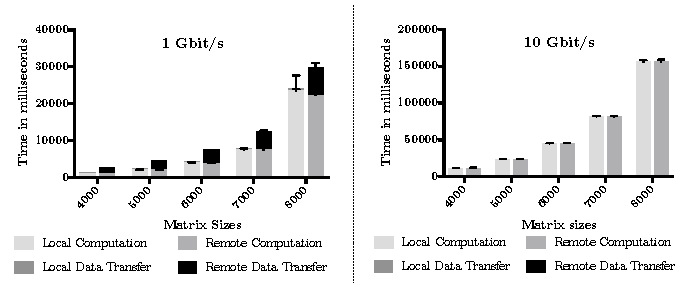
\includegraphics[width=1.0\textwidth]{images/data_transfer.pdf}
\centering
\caption{dOpenCL Benchmark Remote vs. Local}
\label{img:data_transfer}
\end{figure}

It is visible from the obtained results that the local executions have minimal transfer times for the matrices as the only limiting factor is the bus interface between CPU and RAM. One the opposite, data transfers can have significant impact on performance for remote executions as the Ethernet transfers has to be added on top. This is especially true for fast machines that only have an inadequate interconnection speed like Machine B. While for matrix sizes of 8000x8000 the local execution only requires less than 2\% of the time for data transfers, its remote counterpart uses 25\% of the total. In the case of Machine C, the remote transfers profit from the 10 Gbit/s interconnect. As Machine C is considerably slower than Machine B during the computation phase, the fraction of data transfer time from the total is negligible.

Based on the results, one can conclude that the remote computation itself is nearly as fast as the local execution and that the introduced overhead by dOpenCL is marginal. Real performance degradations occur when data transfers have to be processed, which are directly affected by the network performance. Still, dOpenCL can greatly improve performance when accessing a superior machine via remote as seen in the example of Machine C and Machine B. In the given benchmark Machine A could profit from outsourcing the computation of 8000x8000 matrices to Machine B through a 5x speedup\footnote{Considering that Machine A and Machine C have identical setups and therefore assuming that both display equal performance.}.

\section{High-Level Abstraction}
\label{abstraction}

In section \ref{aparapi} it was shown how little code and knowledge of internals are required for building OpenCL computations with the help of Aparapi. Including the library in the eventual framework would not only benefit end users due to a simplified programming environment but also greatly assist during the creation of the framework itself. Through Aparapi Java could be used as the overall language of project while abandoning C++ for most parts with the exception of dOpenCL. Due to the choice of a more high level language for the less performance critical code, Java promises faster building time and better maintainability. In order to achieve this, Aparapi has to be connected to dOpenCL to harness the distribution capabilities. First, it has to be evaluated, whether Aparapi performs adequately compared to an original OpenCL algorithm. For that cause the matrix multiplication benchmark from section \ref{distribution} was transformed to Aparapi and executed on Machine C from the benchmark cluster. As Aparapi translates the Java code for Kernels it has not encountered before, the translation time would skew the results for the first iteration of a run. Therefore at first the translation time for differently sized Kernels was measured on Machine C with 100 iterations per Kernel:

\begin{figure}[H]
	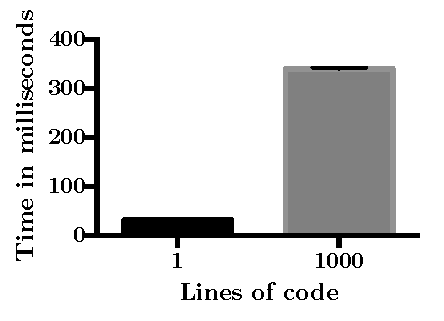
\includegraphics[width=0.5\textwidth]{images/aparapi_translation.pdf}
	\centering
	\caption{Average Kernel translation time}
	\label{img:aparapi_translation}
\end{figure}

It is visible that the translation time of a kernel has a lower bound of ~30ms on Machine C. Additionally it can be concluded that the translation time is correlated to the Kernel size but even for many lines of code remains at around 350ms. In the light of long running computations this time becomes diminishable. Because the translation shall be ignored in the final results an initial run is executed to translate the Kernel before running the measured iterations. The matrix sizes as well as the number of iterations is identical to the benchmark from section \ref{distribution}.

\begin{figure}[H]
	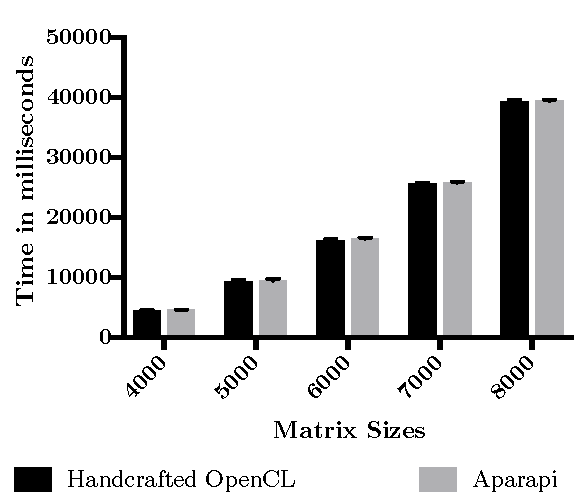
\includegraphics[width=0.5\textwidth]{images/aparapivsopencl.pdf}
	\centering
	\caption{Aparapi vs. Handcrafted OpenCL}
	\label{img:aparapi_vs_opencl}
\end{figure}

As visible in the results, Aparapi can reach the performance level of handcrafted OpenCL code, which for the most runs only takes 1-2\% longer to compute. This minuscule difference could be the result of communication overhead through the JNI interface. Because of the similar performance it is valid to utilize Aparapi in the envisioned framework. As a first step the connection between Aparapi and dOpenCL should be evaluated. For this cause both components were installed in a development system and tested for interoperability. It was discovered that in their standard versions both pieces of software do not work in conjunction because of several bugs or design decisions. These problems and the corresponding solutions will be explained in the following part:

\begin{description}[style=nextline]
	\item [No available devices]
	When querying dOpenCL for appropriate devices from Aparapi, none would be returned even though multiple devices were available when using standard OpenCL. The problem for this symptom lies within dOpenCL, which insufficiently implements the query method. OpenCL uses a single byte to identify queried devices types. For instance \textit{00000010} queries CPUs and \textit{00000100} asks for GPUs. dOpenCL checks for the position of the bit and would correctly return devices of the requested task. The OpenCL standard also allows bitwise OR-operations on multiple types so that when requesting for CPUs and GPUs in one query: \textit{00000010 OR 00000100 = 00000110}. As Aparapi only supports CPUs and GPUs, it specifically asks for these devices even when the user only requests a CPU - filtering the CPUs is then done in Java. Because dOpenCL does not support these combined queries, it can not return any devices to Aparapi. Therefore this method was fixed, which resulted in Aparapi successfully obtaining information about available devices.
	
	\item [Specific device choice]
	Aparapi by design is focused on providing a simple API, which lacks certain features that are important for the framework. For example it is desirable to have multiple instances of the same Kernel run in parallel with different data. Therefore it would be possible to split tasks into smaller subsets of data that could be distributed to various devices. Aparapi allows to define preferences on which specific device a Kernel should be run. This preference is saved on class level instead of instance level, which means that all instances of the same class would be directed to the same device. Therefore no parallelization is possible with the standard Aparapi version. In order to fix this issue, the mechanism for memorizing preferences was modified to respect the definitions for each individual instance of a Kernel.
	
	\item [Failed compilations when using multiple devices]
	Due to fixing the previously described issues, the development system was able to successfully execute Kernels on a single node cluster. Adding a second machine with different installed devices produced an error during the OpenCL compilation process even when only one device was targeted for execution. In the given environment both nodes by itself were able to compile the Kernel without any incidents. Additionally it was verified that dOpenCL without Aparapi supported the multi node cluster. Therefore it was suspected that Aparapi had a bug that prevented the compilation when more than one machine was present. Through reviewing Aparapi internals the cause for the issue was found: Aparapi creates an OpenCL context not per device but per type. OpenCL contexts serve for sharing memory and control structures between multiple devices but can only be defined for devices of the same platform. Thus, when having multiple CPUs of different vendors in a cluster, Aparapi tries to create a context for all CPUs, which creates the error. In order to prevent this violation, in the fixed version contexts are created only for a single device.
	
\end{description} 
 

\section{Job Design}
\label{job_design}
With the implemented fixes described in section \ref{abstraction} Aparapi is able to successfully communicate with dOpenCL and deploy tasks to multiple remote devices. This ability enables jobs to be split up into subtasks, which can be computed in parallel. Therefore the envisioned framework has to provide a mechanism for submitting split tasks by the programmer. With such a mechanism the challenge arises how to distribute data among splits. While some problems may have no or little dependency across data, others may require complex interconnections between individual data points. Thus it is inevitable to ensure that each split has all the necessary data for its correct computation. On the opposite, naively including the full data set in each split may lead to serious performance penalties due to longer data transfer times. This becomes especially important with the introduction of remote execution libraries like dOpenCL, where the most likely bottleneck is the network connection.

Based on previous research the following methods were identified:

\begin{description}[style=nextline]
	\item [Manual Splits]
	Hadoop MapReduce enforces saving input data for the executable tasks in split files on the Hadoop Distributed File System. Each split file is executed independently and programmers have to define how to interpret a split during the map phase. Ultimately, the individually programmed reduce algorithm merges the splits together to form a final result.
	
	\item [Naive Buffer Replication]
	A simple and safe way to ensure that every split has the required data available is to transfer all data to the employed devices as done by \citeauthor{delalama_2012}\cite{delalama_2012}. Their method of buffer replication is trivial when transferring to the devices. On the opposite merging the individual output buffers back into the final result requires an algorithm to determine the parts that should be included by each split.
	
	\item [Intelligent Buffer Replication]
	\citeauthor{Kim_2011}\cite{Kim_2011} have developed a mechanism to automatically determine how to split input buffers among subtasks in OpenCL so that only minimal data has to be transferred. Their method is based on sampling memory access patterns before sending the data so that lower and upper memory bounds can be determined.
		
	\item [Meta Functions]
	\citeauthor{stepocl}\cite{stepocl} as well as \citeauthor{distcl}\cite{distcl} employ meta functions that are utilized to determine split data independent from the problem size. These meta functions have to be supplied by the programmer and define the memory access patterns by the algorithm.
	
\end{description} 

While all of the above mentioned methods are meaningful candidates, they each have negative impact either on performance or programming complexity: \textit{Naive Buffer Replication} increases total data transfer sizes, which enhances the chances of network congestion the higher the number of splits becomes. \textit{Intelligent Buffer Replication} requires an extra step for sampling memory accesses, which includes the translation of OpenCL to C code. Although \textit{Meta Functions} try to abstract efforts away from programmers they are still required to define the access patterns manually. \textit{Manual Splits} put the entire responsibility into the hands of the programmer who has to make sure that the data is split and merged back together. While it is the least automated method, it also grants full control over performance and is not dependent on split and merge algorithms that may fail for complex problems. Thus, the framework will support \textit{Manual Splits}. In order to show that such an approach is eligible in combination with Aparapi the following code example will illustrate the process of splitting the addition of two arrays into subtasks:

\begin{lstlisting}
public class AdditionKernel extends Kernel{
  int[] a, b, result;

  public AdditionKernel(int[] a, int[] b) {
    this.a = a;
    this.b = b;
    this.result = new int[a.length];
  }

  @Override
    public void run() {
    int i = getGlobalId();
    result[i] = a[i] + b[i];
  }
}

public class Addition {
  public static void main(String[] args) {
    final int tileCount = 2;
    int[] a = new int[]{0, 1, 2, 3, 4, 5, 6, 7, 8, 9};
    int[] b = new int[]{0, 1, 2, 3, 4, 5, 6, 7, 8, 9};
    int[] result = new int[a.length];

    int tileWidth = a.length / tileCount;
    for(int i = 0; i < tileCount; i++){
      int[] aTile = Arrays.copyOfRange(a, i * tileWidth, (i + 1) * tileWidth);
      int[] bTile = Arrays.copyOfRange(b, i * tileWidth, (i + 1) * tileWidth);

      AdditionKernel additionKernel = new AdditionKernel(aTile, bTile);
      additionKernel.execute(tileWidth);
      System.arraycopy(additionKernel.result, 0, result, i * tileWidth, tileWidth);
    }

    System.out.println(Arrays.toString(result));
  }
}

\end{lstlisting}

In the example a reusable Aparapi Kernel \textit{AdditionKernel} is defined that computes the sums of the two arrays independent of the general problem size. In the class \textit{Addition} the generated input data is split into smaller parts based on the \textit{tileCount}. Then for each tile the \textit{AdditionKernel} is instantiated and executed. After the execution the individual result is copied into the overall \textit{result} array. In order to grant higher parallelization the \textit{tileCount} could be dynamically changed into a divisor of the array length. This illustrates that writing a split and merge algorithm can be intuitive and not require much code. Additionally, other approaches like \textit{Meta Functions} would still require a substantial amount of code.

explain job/task relation and how Dynamo deals with it

explain how tasks are puts on devices

iterative jobs

design considerations and limitations of Aparapi

\section{Hybrid Cloud}

In the previous sections benchmarks and code examples were shown based on the existence of a local cluster.
While local clusters may provide cheap and stable performance when completely utilized. In reality resource demands fluctuate, making it hard to reach an equilibrium with a full resource utilization and no job queue. For instance, the New York University published monthly utilization measurements for their three clusters in 2013\cite{nyu}, which are shown as a yearly aggregate in table \ref{table:cluster_utilization}. Aside from visible differences in average utilization all clusters show a considerably high standard deviation.

\begin{table}[!htb]
	\centering
	\begin{adjustbox}{width=0.5\textwidth}
		\small
		\begin{tabular}{l | l | l | l}
			~						& Cluster 1	& Cluster 2	& Cluster 3                 \\
			\hline
			Average Utilization 	& 81.1\%  	& 71.0\% 	& 76.1\% \\
			Std. Deviation          & 5.2\%  	& 4.9\%		& 16.9\% \\
		\end{tabular}
	\end{adjustbox}
	
	\caption{NYU Cluster Utilization}
	\label{table:cluster_utilization}
\end{table}

When providing a shared cluster that can be used by multiple parties, certain trade-offs apply. On the one hand overprovisioning decreases waiting times for users but increases costs and reduces utilization. On the other hand underprovisioning reduces costs and may lead to a 100\% utilization but comes with the price that users may have to line up in queues to access resources. Countering this trade-off comes the possibility to employ remote machines from cloud services, which can be booked and released dynamically and are billed hourly or even minutely. Among the most prominent services are Amazon's Elastic Compute Cloud (abbrv. EC2), Microsoft's Azure and Google's App Engine. While each cloud offer by the major players has its advantages and disadvantages, EC2 is the only that has bookable GPU instance types at various sizes. Although Azure and App Engine also have similar offerings, they are either only available as a preview in limited regions or can only be accessed by companies. Therefore, EC2 will be used as the exemplary cloud service for this research but with interchangeability in mind so that it is possible to replace EC2 with other services in the future.

Interconnecting the framework with EC2 requires including the AWS software development kit (abbrv. SDK), which is available for Java among many other languages. Through the SDK, the API for reserving and releasing instances can be accessed. Additionally, an Amazon Machine Image (abbrv. AMI) is required so that newly launched instances will have OpenCL installed and run the dOpenCL daemon by default on startup. For this cause an Ubuntu 14.04 based image was created with the appropriate drivers and dOpenCL installed, which is started right after booting the machine.

Ordering and releasing machines within the framework shall be handled by a class called \textit{Machine Manager}, abstract the actual implementation of the utilized SDK in order to enable users to interchange the underlying cloud provider:


\begin{lstlisting}
public abstract class MachineManager {
  protected abstract List<DynamoInstance> bookInstance(int count, String type);
  protected abstract void terminateInstances(List<DynamoInstance> instances);
  ...

  public List<DynamoInstance> book(int count, String type){
    List<DynamoInstance> instances = bookInstance(count, type);
    ...
    return instances;
  }

  public void release(List<DynamoInstance> instances){
    terminateInstances(instances);
    ...
  }
}
\end{lstlisting}

The above code shows the abstract class that handles bookings and releases of instances in the context of dOpenCL. In the actual implementation it includes functionalities which ensures that the booked instances are successfully booted and running the dOpenCL daemon before adding them to the cluster as well as removing them. These pieces have been deducted for the sake of readability. The actual implementation of the EC2 \textit{Machine Manager} that accesses the SDK is hidden behind the abstract class so that users only communicate with the generalized class. In order to employ another cloud provider, only the abstract methods have to be implemented that call the respective cloud API.

An important factor to consider when connecting a local cluster with a remote cloud is security. Remote machines should be sufficiently secured to prevent attackers from taking over machines or utilizing resources via calling the running dOpenCL daemon. By default the EC2 Ubuntu images only allow certificate based SSH, which prevents password attacks on any account. Additionally, Amazon offers the management of Security Groups that put machines behind a virtual firewall. Therefore the security group can be configured to only allow packages from the static IP range of the local cluster, which renders attacks from outside of the local network useless. Any newly booked instance will be included within the Security Group and as such automatically protected.

\section{Scalable Performance}

In section \ref{job_design} the general job design was explained that is employed in the framework. As jobs may contain an arbitrary number of tasks, this number determines the potential for parallelization. The limit exists as every task is only executed on a single device. For example a matrix multiplication that has been split into four tasks may be computed by four devices in parallel and as such can benefit from a maximum four times speedup based on Amdahl's law. Choosing the appropriate number of tasks is influenced by a performance trade-off: while an increased number of tasks per job offers a greater parallelization and as such a potentially higher performance each task has to be scheduled by the framework and started in its own OpenCL Kernel. Thus, for certain jobs it may be beneficial to keep the number of tasks lower than the number of available devices in the cluster in order prevent performance penalties through overheads.

The general idea behind scaling performance within the framework is based on booking additional resources through a remote cloud when demand is high. Similarly, in the case of low demand resources can be released again in order to minimize costs. Widely employed cluster resource management solutions like Hadoop YARN include functionalities to add or remove nodes dynamically. In a YARN cluster each node is independent and communicates with a central master node that keeps track of utilized resources and handles each compute node as an individual entity. Offering a similar functionality in a dOpenCL based solution differs substantially:

OpenCL and Aparapi were built to run on a single machine and as such include assumptions of limited capabilities concerning changing hardware during operation. For example Aparapi caches device queries to OpenCL as devices are usually added or removed during maintenance procedures when a machine is powered down. dOpenCL overcomes such limitations and enables the central machine to have devices virtually installed by adding nodes to the dOpenCL cluster. dOpenCL therefore extends the OpenCL standard by adding the custom methods \textit{clCreateComputeNodeWWU} and \textit{clReleaseComputeNodeWWU}. 

As OpenCL itself has no multi-machine capabilties it only offers information for the respective built-in devices through the standard API. Therefore all devices appear as if they were installed in the central machine that runs the dOpenCL library. This makes identifying the owning machine per device impossible. Without the relation between devices and machines it can not be ensured that a machine meant to be released is not running any tasks. In order to provide the machine-device relation dOpenCL introduced another method called \textit{clGetDeviceIDsFromComputeNodeWWU}.

The mentioned dOpenCL methods are available to C++ programmers when including the respective header files that contain the extensions. Thus, host code that wants to benefit from dynamic device management has to be modified appropriately. In its standard version Aparapi is bound to the OpenCL standard and has no understanding of the offered dOpenCL extensions. Therefore it is necessary to modify the Aparapi JNI to enable dynamic resource scaling. In order to do so, two new JNI methods are introduced, \textit{addNode} and \textit{removeNode}. Both call the respective dOpenCL functions, with \textit{addNode} also reporting back the available devices of the added node.

introduce general scaling idea based on the job design

show the necessary changes towards dopencl and aparapi

\section{Optimized Scheduling}

As Dynamic OpenCL is supposed to offer its services to variously structured jobs in parallel, scheduling considerations have to be undertaken to maximize overall system efficiency and ensure a fair resource sharing process. It must be understood that both requirements can be contradictory depending on the submitted workloads and heterogeneity of available devices. For instance granting each job the same amount of devices in every scheduling round could mean that some jobs are assigned inadequate devices for their kind of task. For example a job that runs especially well on GPUs could receive a CPU device, thus lowering the overall efficiency. On the other hand, considering only performance based factors might starve certain jobs until all other workloads have finished.

For a flexible approach that can be configured on the respective requirements of the cluster a pluggable two tiered scheduling architecture is proposed. This enables administrators to combine scheduling algorithms based on the requirements of the system. 

\subsection*{Job Scheduling}
The first scheduling tier only considers the system state on a job abstraction level without having any knowledge about the actual task structure or available devices in the cluster. Instead this tier is mainly concerned about ensuring predefined fairness policies and as such controls which jobs are eligible for sending their workloads to the next scheduling tier. Exemplary algorithms for this tier are the following:

\begin{description}[style=nextline]
	\item[First-In First-Out (abbrv. FIFO)] 
	Jobs are fully prioritized by their submission time. Thus, tasks of two jobs will be completely submitted sequentially with the older job coming in front. Example: Job A with two tasks a and Job B with four tasks b will lead to the order aabbbb.
	\item[Round-Robin] 
	Tasks are put equally in rotating order so that each job gets a fair share of resources. Example: Job A with two tasks a and Job B with four tasks b will lead to the order ababbbb.
\end{description}

All of the above approaches do not require insight into the actual performance figures but determine the resulting task order by high level attributes like job submission time etc. Moreover, the selected algorithm on this tier can lead to significantly different outcomes for the overall system due to severe variations in fairness. Still, the first tier only hands over the task order to the second tier, which may be completely ignored based on the nature of the underlying algorithm.

[TODO: explain why scheduler should send more than one job even in fifo]

\subsection*{Device Scheduling}
The second scheduling tier gets its input from the preceding tier and has no concerns of the high level job abstraction. Instead it focuses on the actual assignment of tasks to devices. Executing OpenCL code in a heterogeneous environment can lead to drastically different performance numbers based on the implementation and the executing device. For example code that may perform exceptionally well on a GPU may run poorly on a CPU because of varying computational capabilities. Therefore programmers should be empowered to express preferences in terms of the device types that their algorithm should be computed on. Such functionality is included in the framework through a defined \textit{Device Preference} attribute that can be attached to every task. Valid values for the attribute include: \textit{None}, \textit{CPU only}, \textit{CPU preferred}, \textit{GPU only} and \textit{GPU preferred}. With these five preference levels programmers can accordingly specify their favorite device type. Using the \textit{CPU only} or \textit{GPU only} values signals algorithms to only assign the specific type. On the other hand \textit{CPU preferred} and \textit{GPU preferred} indicate that it is appropriate to schedule a GPU or a CPU respectively if the preferred type is not available. While it is possible for schedulers on this tier to ignore the defined preference, all currently implemented solutions within the framework adhere to the specification. As such the included \textit{Device Preference Scheduler} is the most basic algorithm following the specification. It takes the given tasks one by one and assigns it to the first unutilized matching device that is available.

It must be noted that algorithms on the second tier may utilize entirely different approaches to assign tasks to devices. While it might be feasible in certain environments to randomly send tasks to devices, more thoughtful approaches may improve the overall efficiency of the system. As more analytical algorithms are likely to focus on performance indicators, the most promising options will be explained and evaluated based on their eligibility.

For decades it has been a significant challenge to foresee execution times of algorithms on a given system. Execution times are especially considered in real time systems such as cars, airplanes or space probes where it is mandatory to ensure that an algorithm finishes under a specified boundary, called worst case execution time (abbrv. WCET). In order to obtain such timings one may employ various methods such as static code analysis or simulations\cite{wcet}.

In static code analysis algorithms are taken apart for the purpose of predicting control flow features such as loop counts without executing the actual code\cite{loopbound}\cite{sweet}. While there are formal approaches to gain insights about the executable instructions, estimating the running time is another great challenge. As modern processors have become increasingly complex due to the introduction of caches, pipelines and multi core architectures, instruction times may vary significantly\cite{wcet}. In the light of OpenCL this step becomes even more difficult through the availability of different device types and vendors, which inherit distinct architectures.

Simulations allow to draw conclusions about algorithm timings by running it on an abstract representation of the actual hardware\cite{wcet}. While \citeauthor{multi2sim} have proposed a framework for simulating CPUs and GPUs\cite{multi2sim}, the main drawback of such an approach is again the abundance of different hardware designs and architectures supported by OpenCL. In order to cover the majority of possible devices, many different simulators would be required. For instance, each NVIDIA GPU architecture would demand a dedicated simulator.

While code analysis and simulation do not employ the actual hardware, benchmarks may be used to obtain indicators about the performance of a specific device for a given task. For instance, \citeauthor{quantitative_performance} have proposed a model in which they measure key performance indicators like buffer bandwidth of a GPU\cite{quantitative_performance}. These measurements are then used to predict execution times of Kernels based on the identified bottlenecks by analyzing the instructions at hand. Other approaches run the Kernels with varying parameters in order to infer the dominant performance factors\cite{gpgpu_performance}.

All of the presented approaches are promising in their respective field of application. Still, the major limiting factor is the apparent focus on a specific architecture, which makes the utilization too complex in the context of OpenCL. In order to cover all supported devices many different models would have to be employed, with each upcoming hardware architecture also introducing new models to Dynamic OpenCL.

With the distribution of tasks across a network not only the performance of the execution devices matters but also the speed of the network connection itself. This becomes especially important when utilizing resources from a distant cloud, which inherently can not offer the same bandwidth and latency as a local network. For example, in a benchmark a local cluster with 10 Gbit/s interconnects installed could only reach bandwidths of 190 Mbit/s when communicating to a small EC2 instance. Still the EC2 instance was able to transfer data at the speed of ~800 Mbit/s to second EC2 instance. Thus both machines perform well in their respective local network but the interconnection between the two networks becomes the bottleneck. Such asymmetric connections could significantly affect data intense Kernels where the data transfers might exceed computation times on a slow connection. Thus, sending such Kernels to a high performance cloud device could be worse than sending it to a slower local machine.

A naive approach that combines both measurements for device performance as well as network performance is the usage of historical data. With the assumption that jobs are split in many equally sized tasks one can presume the best suited device of a Kernel from previous runs on various devices within the cluster. As Dynamic OpenCL schedules only a single task on a device at a time, tasks do not interfere with one another performance wise. Therefore the execution time of a Kernel is not affected by other Kernels and should accordingly remain stable across multiple runs. This behavior could also be observed during the benchmarks in section \ref{distribution} and \ref{abstraction} where multiple runs of the same Kernel showed little standard deviations.

In order to offer algorithms on the second tier valuable data, several analytical features are added to Aparapi and Dynamic OpenCL:
\begin{description}[style=nextline]
	\item[Kernel Data Size] 
	Aparapi is extended by adding a method to the Kernel class that reports back the actual size of the overall Kernel including its data. The size is gained by employing Java reflection and thus identifying used data types and data structures. As Aparapi offers explicit memory management not all of the data of a Kernel must be transferred. Analyzing the surrounding Java code to identify the respective memory management calls from within the Kernel is impossible. Therefore the returned size value can only act as an approximation for the real sum of transferred data.
	\item[Historical Data Transfer] 
	While knowing the exact amount of transferable data beforehand in the context of explicit memory management is impossible, retaining these values in the aftermath of a Kernel execution is feasible. For this cause the memory management calls of Aparapi are modified to accumulate the size of the supplied data structure in a Kernel attribute. With this functionality the total amount of transferred data is available after a Kernel has been executed. Then the attribute can be utilized by schedulers to conclude decisions for future Kernels of the same job.
	\item[Performance Cache]
	Dynamic OpenCL implements a mechanism to retain execution times of Kernels for every device it was run on. The observed timespan reaches from the deployment of the Kernel from its host code until the end of execution, thus including network transfers. Therefore the measurement takes into account different locations of the devices within the network. This means that a cloud device should yield slower execution times than a similar local device due to the data transfer penalties. With the resulting data schedulers can conclude decisions either based on individual devices or grouped by model.
\end{description}

Based on the implemented \textit{Performance Cache} the \textit{Performance Based Device Scheduler} is included in Dynamic OpenCL, which assigns the currently available device with the best historical performance to a task. With the available features concerning data transfer analysis more sophisticated and fine grained schedulers are possible to be implemented in the future. Additionally, system wide optimizations are feasible, which minimize the overall execution time of all submitted tasks. For instance, a Simplex algorithm based scheduler would take into account trade off scenarios where it is beneficial not to grant a task its best suited device but minimize the expected execution time among all scheduling decisions. 

It must be noted that schedulers on this tier may rightfully ignore the order of tasks given by the first tier. For example the first tier might hand over a list of tasks in FIFO order. If this list is handled by a Simplex based scheduler on the second tier, the principle of FIFO may be violated in order to find the optimal distribution.

reason that the second tier may ignore the first one completely, also why fifo isnt necessarily fifo
\section{Exemplary Use Cases}

In the previous sections the main characteristics of Dynamic OpenCL were explained. The included features make it a viable option for a variety of use cases which will be introduced in the following.

\begin{description}[style=nextline]
	\item[Job Based Library]
	One use case for the framework is to utilize it as a Java library for a single job thus keeping management overhead minimal. Programmers can either transform OpenCL code from C or C++ to Aparapi or adapt already existant Aparapi code. In theory Aparapi code can be submitted to Dynamic OpenCL without any changes but would not fit into the required task structure and therefore run in a single Kernel. In order to utilize parallelization, programmers are mandated to split their jobs into smaller tasks and submit those.
	
	With the focus on a single job Dynamic OpenCL can schedule the submitted tasks across a given cluster and report back results. As there are no other jobs to interfere with no extensive scheduling is required and all resources can be freely assigned to said job. In the case of a slower execution than expected users may book additional resources from an implemented cloud service and therefore reduce overall execution time in return for higher costs.
	
	\item[Local Cluster Provider] 
	
	Instead of only acting on behalf of a single job, programmers can utilize Dynamic OpenCL to offer a shared platform for users to submit their jobs to. This becomes especially meaningful in the light of daily recurring jobs that only have to be programmed once. The platform could allow users to submit data to predefined jobs that take care of splitting the data into meaningful chunks. Therefore users can profit from parallelization on powerful hardware without having programming knowledge on their own.
	
	The main limitation of the local cluster provider is its restriction to local resources only. Therefore the platform can not dynamically book instances from a cloud provider and with that increase the overall capabilities of the cluster. Running a shared platform on a local cluster may require some performance based scheduling in order to optimize resource assignments based on the running jobs. Likewise administrators may choose to introduce simpler scheduling algorithms like First In First Out. 
	
	\item[Hybrid Cloud Provider] 
	Local clusters may lead to phases of overprovisioning when resource demands by users are low, thus causing costs without any return in computation. In order to provide a more dynamic infrastructure Dynamic OpenCL can be used to guarantee a baseline of performance through local resources and add devices to the cluster from a cloud service when needed. While cloud devices may be more costly than local resources they can assist during peak demands and be released afterwards. Hence the overall costs of using a cloud resource may be lower than operating an underutilized local device.
	
	Additionally, volatile hardware requirements may lead to high total costs of ownerships. For instance, if only one job per month requires a GPU for efficient execution, installing a GPU in the local cluster might be costly. Instead such resources could be employed on demand whenever a job with such requirements is submitted.
	
	The main drawback of a hybrid cluster is the interconnection between both parts of the network that may suffer from low bandwidths. Therefore scheduling algorithms should be utilized that take the hybrid infrastructure into account and assign tasks accordingly.
	
	\item[Cloud Cluster Provider]
	While hybrid clusters unite a static performance baseline with dynamic adjustments based on demand, a completely customizable infrastructure is also possible. Instead of having computational resources running at all times, cloud clusters may only run a single management node. This central node receives jobs and orders new cloud resources depending on the actual demand. At times of no demand the management node runs alone, hence producing minimal costs.
	
	
\end{description}


